\documentclass[a4paper, 11pt, oneside]{article}
\usepackage[svgnames]{xcolor}
\usepackage{graphicx} % Required for box manipulation
\usepackage{geometry}
\usepackage{pgfplots}
\pgfplotsset{compat=1.14}
\geometry{legalpaper, margin=1in}
\newcommand*{\plogo}{\fbox{$\mathcal{PL}$}} % Generic dummy publisher logo

\usepackage[utf8]{inputenc} % Required for inputting international characters
\usepackage[T1]{fontenc} % Output font encoding for international characters
\usepackage{PTSerif} % Use the Paratype Serif font
\usepackage{amsmath}
\usepackage{amssymb}
\usepackage{chngcntr}
\counterwithin*{subsection}{section}
\usepackage{graphicx}
\graphicspath{}

\begin{document}

\begin{center}  % Centre all text
	
	%------------------------------------------------
	%	Title and subtitle
	%------------------------------------------------
	
	\setlength{\unitlength}{0.6\textwidth} % Set the width of the curly brackets above and below the titles
	
	{\color{LightGoldenrod}\resizebox*{\unitlength}{\baselineskip}{\rotatebox{90}{$\}$}}}\\[\baselineskip] % Top curly bracket
	
	\textcolor{Sienna}{\textit{\Huge MAST90045\\ $\;$ \\Systems Modelling and Simulation}}\\[\baselineskip] % Title
	
	{\color{RosyBrown}\Large Assignment 2}\\ % Subtitle or further description
	
	{\color{LightGoldenrod}\resizebox*{\unitlength}{\baselineskip}{\rotatebox{-90}{$\}$}}} % Bottom curly bracket
	
	 % Whitespace between the title and the author name
	
	%------------------------------------------------
	%	Author
	%------------------------------------------------
	
	{\Large\textbf{Chris Swan 370502}}\\ % Author name
	
	
	
	%------------------------------------------------
	%	Publisher
	%------------------------------------------------
	
	%\plogo\\[0.5\baselineskip] % Publisher logo
	
	University of Melbourne % Publisher name

\end{center}

\tableofcontents


\section{Problem Introduction}

Life is filled with hypothetical scenarios that we are constantly trying to understand, sometimes without even realising that we are. Sometimes these can seem trivial, like posing what-if questions about historical events or alternate outcomes of sporting events. However, from these hypotheses can come applications for solving parallel problems that are perhaps not initially apparent. And whilst an initial problem may seem trivial, it can provide the foundations for solving challenges that very much are not. \\

Such is the case with the scenario we are presented. Simulating a game of Squash may seem limited in application to the sporting world, however as we shall see as we delve into the probabilistic aspects of the task, the problem has potential overlap with many other areas. It is not so much the problem itself but the methodology that is used which is the critical thing: in simulating Squash, one might garner an idea of how to simulate a debate between two politicians or how a boxing match might unfold.\\

This problem involves four stages:

\begin{itemize}

\item creating a function to model the status of a game, \textbf{ie} how a point is played

\item simulating a game - that is, how the tallying of points build towards victory for a particular player

\item the probability of a particular player winning given their likelihood of winning a point

\item the estimated average length of a game given a particular player's likelihood of winning a point

\end{itemize}

\newpage
We begin with the following definitions:

\begin{flalign*}
a &= \mathbb{P}(\text{player 1 wins a point } | \text{ player 1 serves})\\
b &= \mathbb{P}(\text{player 1 wins a point } | \text{ player 2 serves})\\
x &= \text{the number of points won by player 1}\\
y &= \text{the number of points won by player 2}\\
z &= \begin{cases} 1 \text{ if player 1 has the serve}\\ 2 \text{ if player 2 has the serve} \end{cases}
\end{flalign*}

\begin{itemize}
\item A player's score increases if they win a point whilst serving; if they lose the point then the serve is transferred to the other player and the scores remain the same.  
\item To win, a player must lead by 2 or more points and reach a minimum score of 9.  A game may continue indefinitely if a 2 point lead is never reached.
\end{itemize}

\section{Status of the game}

The status function is the linchpin upon which the model hangs: if there is a case where this function fails, the rest of the model will likely fail as well. Indeed, in testing we found the we had ordered some of our if statements incorrectly, causing a later function simulating a game being played to loop forever as the model failed to recognise player 2 leading by two points in a tie-break as a win.


\begin{figure}[h]
\centering
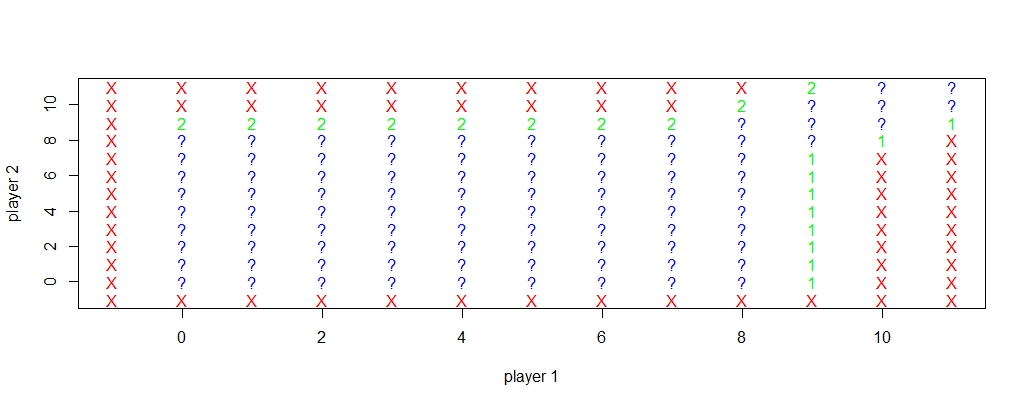
\includegraphics[width=\textwidth]{status}
\caption{Potential status of a Squash game}
\end{figure}

In Figure 1, we see the possible cases for the status of a game. This gives us some assurance that the status function is working correctly - although as seen in our exception discussed above, it does not cover cases beyond the parameters of the graph. The four cases shown are:
\begin{itemize}
\item an impossible scenario (red X)
\item an unresolved scenario (blue ?)
\item player 1 wins (green 1)
\item player 2 wins (green 2)
\end{itemize}

From here we can begin simulating a game.


\section{Simulating a game}

To go about simulating a game, we first define a function to describe the playing of a point.  To do this, we use a Bernoulli distribution for each of the cases where either player 1 is serving or player 2 is serving.  We define a function "play\_point" that inputs the status of play - that is the score and which player is serving - and the probability that player 1 will win the point: either $a$ or $b$, depending on if player 1 or 2 is serving respectively.\\

The function then updates the status and returns it, representing the new state of the game. This function "play\_point" then feeds into the function "play\_game", which loops through iterations of "play\_point", until the updated status is no longer returning 'unfinished' from the "status" function.  \\

This done, the "play\_game" function will either return TRUE if player 1 wins the game or FALSE if not. It is here that another potential flaw in the model can arise: if one fails to properly define 'status', should the status function somehow return 'impossible', "play\_game" will return this as FALSE, which may then be misinterpreted as a win for player 2.\\

We now define $p(a,b) = \mathbb{P}(\text{player 1 wins the game } | \text{player 1 serves first})$, which is recycling our nomenclature of $a$ and $b$ to some degree, but no matter.  As our "play\_game" function has player 1 serving first by default, this serves our purposes for this expression.  \\

We create a function "squash\_prob" for returning the average probability of player 1 winning across $n = 2^k$ games, for $k = 1,2,\dots, 12$.  We see the output of this from our simulation in Figure 2.\\

\begin{figure}[h]
\centering
\begin{tikzpicture}
\begin{axis}[
xlabel={$log_2(n)$},
ylabel={$\hat{p}$},
xmin=0, xmax=12, 
ymin=0.4, ymax=1,
xmajorgrids=true,
ymajorgrids=true,
grid style=dashed
]
\addplot[only marks, blue] table [x=a, y=e, col sep=comma] {
a,e
1,1.0000000 
2,0.7500000 
3,0.7500000 
4,0.6250000 
5,0.5625000 
6,0.5000000 
7,0.4531250 
8,0.4726562 
9,0.5273438 
10,0.5126953 
11,0.5317383 
12,0.5383301
};
\end{axis}
\end{tikzpicture}
\caption{Estimated probability for $log_2(n)$ sample sizes}
\centering
\end{figure}

We are asked whether $p(0.55,0.45) = 0.5$.  One might be forgiven for assuming this to be the case as $log_2(n) \rightarrow \infty$, however this is an oversimplification.  Whilst there appears to be no analytic way to solve the convergence, as one considers averages taken of larger $n$ values, $p(0.55,0.45)$ appears to oscillate around a probability slightly higher than $0.5$: approximately $0.54$, although this is speculative.  Nonetheless, it cannot be concluded that $p(0.55,0.45)$ will converge to $0.5$.

\section{Probability of winning}

\subsection*{Bernoulli Distribution}
For a single Bernoulli random variable, we have by definition:

\begin{flalign*}
X & \sim \text{Bernoulli}(p)\\
\mathbb{P}(X &= x)  \begin{cases} p \quad & \text{ for } x = 1;\\ 1-p \quad & \text{ for } x = 1; \end{cases}\\
\mathbb{E}X &= 1 \cdot p + 0 \cdot (1-p)\\
& =p\\
\text{We have that:}\\
\text{Var}X 	&= \mathbb{E}[(X-p)^2]\\
			&= \mathbb{P}(X=1) \cdot (X(1) - p)^2 + \mathbb{P}(X=0) \cdot (X(0) - p)^2\\
			&= p(1-p)^2 + (1-p)(0-p)^2\\
			&= p(1-p)
\end{flalign*}

Therefore, for $n$ independent and identically distributed Bernoulli$(p)$ random variables, Var$X$ will be $n \cdot p(1-p)$.\\

\newpage
For $\hat{p} = \bar{X}$:

\begin{flalign*}
\bar{X} 			&= \frac{1}{n}(x_1 + \cdots + x_n)\\
\text{Var}\bar{X} 	&= \frac{1}{n^2}\text{Var}(x_1 + \cdots + x_n)\\
\text{Given that each } x_i \text{ is iid:}\\
\text{Var}\bar{X}	&= \frac{1}{n^2} \bigg( \text{Var}(x_1) + \cdots + \text{Var} (x_n) \bigg)\\
				&= \frac{n \cdot p(1-p)}{n^2}\\
				&= \frac{p(1-p)}{n}
\end{flalign*}

$$\therefore \text{Var}\; \hat{p} = \frac{p(1-p)}{n}$$



\subsection*{Standard Deviation of $\hat{p}$}

Given that the largest $p$ we can have is $1$:

\begin{flalign*}
\sqrt{\frac{p(1-p)}{n}} &\leq 0.01\\
\sqrt{\frac{1}{n}} &\leq 10^{-2}\\
\frac{1}{n} &\leq 10^{-4}\\
n &\geq 10^4
\end{flalign*}

Therefore an $n$ of $10^4$ will assure a standard deviation of no more than 0.01 across all simulations of estimated $p(a,b)$ for various $a$ and $b$.\\

\subsection*{Estimated $p(a,b)$}

We find these estimated probabilities for $p(a,b)$ below in Table 1:\\


\begin{table}[h]
\centering
\begin{tabular}{r|rrrrrrrrr}
 & a=0.1 & a=0.2 & a=0.3 & a=0.4 & a=0.5 & a=0.6 & a=0.7 & a=0.8 & a=0.9 \\ 
  \hline
  b=0.1 & 0.00 & 0.00 & 0.00 & 0.00 & 0.00 & 0.00 & 0.01 & 0.05 & 0.50 \\ 
  b=0.2 & 0.00 & 0.00 & 0.00 & 0.00 & 0.01 & 0.04 & 0.16 & 0.51 & 0.95 \\ 
  b=0.3 & 0.00 & 0.00 & 0.01 & 0.03 & 0.08 & 0.23 & 0.52 & 0.85 & 1.00 \\ 
  b=0.4 & 0.00 & 0.02 & 0.05 & 0.13 & 0.28 & 0.51 & 0.79 & 0.96 & 1.00 \\ 
  b=0.5 & 0.02 & 0.06 & 0.15 & 0.31 & 0.54 & 0.77 & 0.93 & 0.99 & 1.00 \\ 
  b=0.6 & 0.06 & 0.17 & 0.34 & 0.54 & 0.74 & 0.91 & 0.98 & 1.00 & 1.00 \\ 
  b=0.7 & 0.17 & 0.36 & 0.56 & 0.75 & 0.89 & 0.97 & 0.99 & 1.00 & 1.00 \\ 
  b=0.8 & 0.36 & 0.59 & 0.78 & 0.90 & 0.97 & 0.99 & 1.00 & 1.00 & 1.00 \\ 
  b=0.9 & 0.65 & 0.83 & 0.93 & 0.97 & 0.99 & 1.00 & 1.00 & 1.00 & 1.00 \\ 
\end{tabular}
\caption{Estimated $p(a,b)$ for various $a$ and $b$}
\end{table}

There are a couple of things to note here.  We see in both the top left quadrant and the bottom right quadrant that player 2 and player 1 are respectively assured to win.  This is to be expected when a player has an extremely high probability of winning a point, regardless of who serves.  \\

What is significant is the sudden increase for $a=0.1, b=0.9$, compared with $a=0.1, b=0.9$. Player 1 goes from having a 5\% chance of winning to a 50\% chance.  There is a similar jump in the bottom left corner, although not as drastic.  The fact that the score increases when a player wins a point on their serve is significant here because player 1 begins with the serve, and is therefore more likely to be able to score points, with a 90\% chance of winning their serve.\\

It is also interesting how the probabilities remain similar along most minor diagonals (moving from the top right to the bottom left), and that when they change they do so only slightly.  We see the larger values in the bottom left quadrant (where player 1 is more likely to win when serving) as indicative of the higher estimated probability of player 1 winning games.


\section{Length of a game}

We modified the "play\_game" function to count the length of a game played, rather than recording the outcome.  These game lengths were then averaged across the same parameter $n=10^4$ as the estimated probabilities were in Table 1.  We see these average game lengths for various $a$ and $b$ below in Table 2:\\


\begin{table}[h]
\centering
\begin{tabular}{r|rrrrrrrrr}
 & a=0.1 & a=0.2 & a=0.3 & a=0.4 & a=0.5 & a=0.6 & a=0.7 & a=0.8 & a=0.9 \\ 
  \hline
   b=0.1 & 12.21 & 14.85 & 18.29 & 22.80 & 28.98 & 38.59 & 54.48 & 85.60 & 151.30 \\ 
   b=0.2 & 12.49 & 15.30 & 18.97 & 23.74 & 30.34 & 40.24 & 55.00 & 74.16 & 84.65 \\ 
   b=0.3 & 12.83 & 15.88 & 19.79 & 24.81 & 31.48 & 39.69 & 48.62 & 53.97 & 53.27 \\ 
   b=0.4 & 13.29 & 16.53 & 20.55 & 25.35 & 30.79 & 35.98 & 38.98 & 39.10 & 37.51 \\ 
   b=0.5 & 13.84 & 17.18 & 20.96 & 24.83 & 28.05 & 30.19 & 30.33 & 29.21 & 27.98 \\ 
   b=0.6 & 14.40 & 17.54 & 20.48 & 22.81 & 23.97 & 24.13 & 23.43 & 22.49 & 21.67 \\ 
   b=0.7 & 14.67 & 17.22 & 18.83 & 19.59 & 19.66 & 19.08 & 18.37 & 17.72 & 17.18 \\ 
   b=0.8 & 14.30 & 15.61 & 16.05 & 15.94 & 15.50 & 14.93 & 14.45 & 14.07 & 13.76 \\ 
   b=0.9 & 12.59 & 12.81 & 12.60 & 12.30 & 11.94 & 11.63 & 11.41 & 11.24 & 11.10 \\ 
\end{tabular}
\caption{Average length of a game for various $a$ and $b$}
\end{table}

We again observe interesting patterns along the minor diagonals.  Working down towards the bottom left corner, we see the lengths of games descending.  Again we see an interesting region of scenarios in the top right corner, with games going in excess of 50 points - and indeed up to 151 for $a=0.1, b=0.9$.  It is notable that game lengths do not appear to relate to win probabilities.  Were one given either Table 1 or Table 2, it would do not be feasible to calculate the elements of the other.\\

It is also interesting that even when probabilities of player 1 winning are $1$, game lengths can still go up to 50 points, as is the case for $a=0.3, b=0.9$.  Here, the serve will be changing many times in a game, as the probability for both players to win their serve is low.  However, in the bottom right corner (when the server is likely to win their serve), games are relatively short.

\section{Summary}

In reviewing our analysis of the many simulations of Squash games, it is noteworthy that something that appears straightforward and simple to an undiscerning eye can be so probabilistically nuanced.  One should also note the lack of absolute precision at work: there exists no analytic method to obtaining these probabilities, and whilst the methods used may not have been overly complex, without mechanical computation the above task would have been impossible.  Finally, we again make the point that the above exposition is demonstrative of what can be explored with simulation and mathematical modelling.



\newpage

\section{Appendix: Code}

\begin{verbatim}
## Assignment 2: A Game of Squash


rm(list=ls())

####################################################

## ___ Status of the game ___


status = function(x,y) {
  #' for integer inputs x and y, returns:
  #' 
  #' 'unfinished' if the game has not yet finished; 
  #'  
  #' 'player 1 win' if player 1 has won the game; 
  #' 
  #' 'player 2 win' if player 2 has won the game; 
  #' 
  #' 'impossible' if x and y are impossible scores. 
  
  im = 'impossible'
  p1 = 'player 1 win'
  p2 = 'player 2 win'
  un = 'unfinished'
  
  if (x < 0 | y < 0) return(im)
  
  if (x == 9 & x - y > 1) return(p1)
  else if (x > 9 & x - y == 2) return (p1)
  
  if (y == 9 & y - x > 1) return(p2)
  else if (y > 9 & y - x == 2) return(p2)
  
  if (x > 9 & x - y > 2) return(im)
  if (y > 9 & y - x > 2) return(im)
  
  else return(un)
}


# From the spuRs library:

# Program spuRs/resources/scripts/status.test.r

status.test <- function(s.ftn) {
  
  x.vec <- (-1):11
  y.vec <- (-1):11
  plot(x.vec, y.vec, type = "n", xlab = "x", ylab = "y")
  
  for (x in x.vec) {
    for (y in y.vec) {
      s <- s.ftn(x, y)
      if (s == "impossible") text(x, y, "X", col = "red")
      else if (s == "unfinished") text(x, y, "?", col = "blue")
      else if (s == "player 1 win") text(x, y, "1", col = "green")
      else if (s == "player 2 win") text(x, y, "2", col = "green")
    }
  }
  return(invisible(NULL))
}



status.test(status)

####################################################

## ___ Simulating a game ___


play_point = function(state, a, b) {
  #' We simulate a point played based on a binomial distrubition with parameters of 
  #' 1 observation and 1 trial, with probabilities
  #'  'a': the probability that player 1 wins a point if player 1 serves,  or
  #'  'b': the probability that player 1 wins a point if player 2 serves
  #' 
  #' state will be the vector (x,y,z) where x: number of points won by player 1, 
  #' y: number of points won by player 2
  #' z = 1 if player is serving and z=2 if player 2 is serving
  
  if (state[3] == 1) {
    bin1 = rbinom(1,1,a)
    new_state = c( bin1, 0, 1 - bin1 )
  }
  if (state[3] == 2) {
    bin2 = rbinom(1,1,b)
    new_state = c( 0, 1 - bin2, - bin2)
  }
  state = state + new_state
}


# Program spuRs/resources/scripts/play_game.r

play_game <- function(a, b) {
  state <- c(0, 0, 1)
  while (status(state[1], state[2]) == "unfinished") {
    # show(state)
    state <- play_point(state, a, b)
  }
  if (status(state[1], state[2]) == "player 1 win") {
    return(TRUE)
  } else {
    return(FALSE)
  }
}
play_game(0.1,0.7)



MySeed = 3133

squash_prob = function(a,b,n,seed_gen){
  #' For producing the average probability of player 1 wining a game based on probabilities 
  #' 'a' and 'b' as defined above, and on 'n games played
  
  game = c()
  set.seed(seed_gen)
  
  for (k in 1:n) { game[k] = play_game(a,b) }
  
  return(mean(game))
}


p_hat = c()

for (i in 1:12) { p_hat = append(p_hat, squash_prob(0.55,0.45,2^i,MySeed)) }

p_hat

plot(1:12, p_hat, type = 'p', main = "Estimated probability for sample size 'n'", 
                                                      xlab = "log(n)/log(2)", ylab = "p_hat")


####################################################

## ___ Probability of Winning ___


biggest_n = 10^4

A = seq(0.1,0.9,0.1)
B = seq(0.1,0.9,0.1)

est_p_ab = matrix( nrow = 9, ncol = 9 )

for (x in 1:9) { for (y in 1:9) { est_p_ab[x,y] = squash_prob(A[x], B[y], biggest_n, MySeed) }}

View(est_p_ab)

Est = round(est_p_ab,2)

View(Est)

print(xtable(Est))

####################################################

## ___ Length of a Game ___


game_length <- function(a, b) {
  #'the length of a game played (until state not 'unfinished'), with 'a','b' as defined above
  #'
  state <- c(0, 0, 1)
  points_played = 0
  
  while (status(state[1], state[2]) == "unfinished") {
    # show(state)
    
    state <- play_point(state, a, b)
    
    points_played = points_played + 1
    
  }
  return(points_played)
  
}

squash_length_prob = function(a,b,n,seed_gen){
  #' the estimated average game length for 'n' games, with 'a','b' as defined above
  #' 
  game = c()
  set.seed(seed_gen)
  
  for (k in 1:n) { game[k] = game_length(a,b) }
  
  return(mean(game))
}


length_p_ab = matrix( nrow = 9, ncol = 9)

for (x in 1:9) { for (y in 1:9) { length_p_ab[x,y] = 
                               squash_length_prob(A[x], B[y], biggest_n, MySeed)}}

View(length_p_ab)

Len = round(length_p_ab,2)

View(Len)

print(xtable(Len))

\end{verbatim}




\end{document}
